%%%%% --------------------------------------------------------------------------------
%%
%%                               Document Template
%%
%%%%% --------------------------------------------------------------------------------
%% Copyright (C) Huangrui Mo <huangrui.mo@gmail.com> 
%% This is free software: you can redistribute it and/or modify it
%% under the terms of the GNU General Public License as published by
%% the Free Software Foundation, either version 3 of the License, or
%% (at your option) any later version.
%%%%% --------------------------------------------------------------------------------
%%
%%%%************************ Document Class Declaration ******************************
%%
\documentclass[doublesided]{Style/ucasthesis}% thesis template of UCAS
%% Multiple optional arguments:
%% [scheme = plain] % for thesis writing of international students
%% [<singlesided|doublesided|printcopy>] % single-sided, double-sided, or print layout
%% [draftversion] % show draft version information, default is no show
%% [fontset = <adobe|...>] % specify font set, default is automatic detection
%% [standard options for ctex class]
%%%%% --------------------------------------------------------------------------------
%%
%%%%************************* Command Define and Settings ****************************
%%
\usepackage[myhdr]{Style/commons}% common settings
%% usage: \usepackage[option1,option2,...,optionN]{commons}
%% Multiple optional arguments:
%% [<numbered|authoryear|alpha>] % citation and reference style
%% <numbered>: textual: Jones [1]; parenthetical: [1]. default style
%% <authoryear>: textual: Jones (1995); parenthetical: (Jones, 1995)
%% <alpha>: textual: not available; parenthetical: [Jon95]
%% [myhdr] % one available header and footer style, will enable fancyhdr
%% [lscape] % provide landscape layout environment
%% [geometry] % configure page layout by geometry package
%% [list] % enable enhanced list environments, useful for Algorithm and Coding
%% [color] % enable color package to use color, default package is xcolor
%% [background] % enable page background, will auto enable color package
%% [tikz] % enable tikz for complex diagrams, will auto enbale color package
%% [table] % enable a table package for complex tables, default is ctable
%% [math] % enable some extra math packages
\usepackage{Style/custom}% user defined commands
%%%%% --------------------------------------------------------------------------------
%%
%%%%******************************** Content *****************************************
%%
\begin{document}
%%
%%%%% --------------------------------------------------------------------------------
%%
%%%%******************************** Frontmatter *************************************
%%
%% Frontmatter of Title page, Table of contents, Preface chapter.
\frontmatter
%%
%% >>> Frontpages
%%
%%
%%% >>> Title Page
%%
%%
%%% Chinese Title Page
%%
  \confidential{}% show confidential tag
  \schoollogo{scale=0.112}{UCAS}% university logo
  \title[国科大学位论文\LaTeX{}模板]{中国科学院大学学位论文\LaTeX{}模板}% \title[short title for headers]{Long title of thesis}
  \author{莫晃锐}% name of author
  \advisor{刘青泉~研究员}% names and titles of supervisors
  \advisorinstitute{中国科学院力学研究所}% institute names of supervisors
  \degree{硕士}% degree
  \degreetype{理学}% degree type
  \major{流体力学}% major
  \institute{中国科学院力学研究所}% institute of author
  %\chinesedate{2014~年~06~月}% only need for user customized date
%%
%%% English Title Page
%%
  \englishtitle{\LaTeX{} Thesis Template\\ of \\ The University of Chinese Academy of Sciences}
  \englishauthor{Huangrui Mo}
  \englishadvisor{Professor Qingquan Liu}
  \englishdegree{Master}
  \englishthesistype{thesis}
  \englishmajor{Fluid Mechanics}
  \englishinstitute{Institute of Mechanics, Chinese Academy of Sciences}
  %\englishdate{June, 2014}% only need for user customized date
%%
%%% Generate Chinese Title
%%
\maketitle
%%
%%% Generate English Title
%%
\makeenglishtitle
%%
%%% >>> Author's declaration
%%
\makedeclaration
%%
%%% >>> Abstract
%%
\chapter{摘\quad 要}% does not show the title on the top
%\begin{abstract}% will show the title on the top
本文是中国科学院大学学位论文模板ucasthesis的使用说明文档。主要内容为介绍\LaTeX{}文档类ucasthesis的用法,以及如何使用\LaTeX{}快速高效地撰写学位论文。

\keywords{中国科学院大学,学位论文,\LaTeX{}模板}
%\end{abstract}


\chapter{Abstract}% does not show the title on the top
%\begin{englishabstract}% will show the title on the top
This paper is a help documentation for the \LaTeX{} class ucasthesis, which is  a thesis template for the University of Chinese Academy of Sciences. The main content is about how to use the ucasthesis, as well as how to write thesis efficiently by using \LaTeX{}.

\englishkeywords{University of Chinese Academy of Sciences (UCAS), Thesis, \LaTeX{} Template}
%\end{englishabstract}

%%
%%% >>> List of Content
%%
\intotoc{\contentsname}% add a corresponding item to the contents table and bookmark
\tableofcontents% contents catalog
\intotoc{\listfigurename}% add a corresponding item to the contents table and bookmark
\listoffigures% figures catalog
\intotoc{\listtablename}% add a corresponding item to the contents table and bookmark
\listoftables% tables catalog
%%
%% >>> prematter
%%
%%
%% >>> Nomenclatures
%%
\chapter{符号列表}

\section*{Characters}
\nomenclatureitem[\textbf{Unit}]{\textbf{Symbol}}{\textbf{Description}}
\nomenclatureitem[$\Unit{m^{2} \cdot s^{-2} \cdot K^{-1}}$]{$R$}{the gas constant}
\nomenclatureitem[$\Unit{m^{2} \cdot s^{-2} \cdot K^{-1}}$]{$C_v$}{specific heat capacity at constant volume}
\nomenclatureitem[$\Unit{m^{2} \cdot s^{-2} \cdot K^{-1}}$]{$C_p$}{specific heat capacity at constant pressure}
\nomenclatureitem[$\Unit{m^{2} \cdot s^{-2}}$]{$E$}{specific total energy}
\nomenclatureitem[$\Unit{m^{2} \cdot s^{-2}}$]{$e$}{specific internal energy}
\nomenclatureitem[$\Unit{m^{2} \cdot s^{-2}}$]{$h_T$}{specific total enthalpy}
\nomenclatureitem[$\Unit{m^{2} \cdot s^{-2}}$]{$h$}{specific enthalpy}
\nomenclatureitem[$\Unit{kg \cdot m \cdot s^{-3} \cdot K^{-1}}$]{$k$}{thermal conductivity}
\nomenclatureitem[$\Unit{K}$]{$T$}{temperature}
\nomenclatureitem[$\Unit{s}$]{$t$}{time}
\nomenclatureitem[$\Unit{kg \cdot m^{-1} \cdot s^{-2}}$]{$p$}{thermodynamic pressure}
\nomenclatureitem[$\Unit{kg \cdot m^{-1} \cdot s^{-2}}$]{$\hat{p}$}{hydrostatic pressure}
\nomenclatureitem[$\Unit{kg \cdot m^{-2} \cdot s^{-2}}$]{$\Vector{f}_b$}{body force}
\nomenclatureitem[$\Unit{m^2}$]{$\mathrm{S}$}{boundary surface}
\nomenclatureitem[$\Unit{m^3}$]{$\mathrm{V}$}{volume}
\nomenclatureitem[$\Unit{m \cdot s^{-1}}$]{$\Vector{V}$}{velocity vector}
\nomenclatureitem[$\Unit{m \cdot s^{-1}}$]{$u$}{x component of velocity}
\nomenclatureitem[$\Unit{m \cdot s^{-1}}$]{$v$}{y component of velocity}
\nomenclatureitem[$\Unit{m \cdot s^{-1}}$]{$w$}{z component of velocity}
\nomenclatureitem[$\Unit{m \cdot s^{-1}}$]{$c$}{speed of sound}
\nomenclatureitem[$\Unit{m}$]{$\Vector{r}$}{position vector}
\nomenclatureitem[$\Unit{1}$]{$\unitVector{n}$}{unit normal vector}
\nomenclatureitem[$\Unit{1}$]{$\hat{\unitVector{t}}$}{unit tangent vector}
\nomenclatureitem[$\Unit{1}$]{$\tilde{\unitVector{t}}$}{unit bitangent vector}
\nomenclatureitem[$\Unit{1}$]{$C_R$}{coefficient of restitution}
\nomenclatureitem[$\Unit{1}$]{$Re$}{Reynolds number}
\nomenclatureitem[$\Unit{1}$]{$Pr$}{Prandtl number}
\nomenclatureitem[$\Unit{1}$]{$Ma$}{Mach number}
\nomenclatureitem[$\Unit{m^2 \cdot s^{-1}}$]{$\alpha$}{thermal diffusivity}
\nomenclatureitem[$\Unit{kg \cdot m^{-1} \cdot s^{-1}}$]{$\mu$}{dynamic viscosity}
\nomenclatureitem[$\Unit{m^2 \cdot s^{-1}}$]{$\nu$}{kinematic viscosity}
\nomenclatureitem[$\Unit{1}$]{$\gamma$}{heat capacity ratio}
\nomenclatureitem[$\Unit{kg \cdot m^{-3}}$]{$\rho$}{density}
\nomenclatureitem[$\Unit{kg \cdot m^{-1} \cdot s^{-2}}$]{$\sigma_{ij}$}{stress tensor}
\nomenclatureitem[$\Unit{kg \cdot m^{-1} \cdot s^{-2}}$]{$S_{ij}$}{deviatoric stress tensor}
\nomenclatureitem[$\Unit{kg \cdot m^{-1} \cdot s^{-2}}$]{$\tau_{ij}$}{viscous stress tensor}
\nomenclatureitem[$\Unit{1}$]{$\delta_{ij}$}{Kronecker tensor}
\nomenclatureitem[$\Unit{1}$]{$I_{ij}$}{identity tensor}

\section*{Operators}
\nomenclatureitem{\textbf{Symbol}}{\textbf{Description}}
\nomenclatureitem{$\Delta$}{difference}
\nomenclatureitem{$\nabla$}{gradient operator}
\nomenclatureitem{$\delta^{\pm}$}{upwind-biased interpolation scheme}

\section*{Abbreviations}
\nomenclatureitem{\textbf{Acronym}}{\textbf{Description}}
\nomenclatureitem{ANFO}{Ammonium Nitrate Fuel Oil}
\nomenclatureitem{CFD}{Computational Fluid Dynamics}
\nomenclatureitem{CFL}{Courant-Friedrichs-Lewy}
\nomenclatureitem{CJ}{Chapman-Jouguet}
\nomenclatureitem{EOS}{Equation of State}
\nomenclatureitem{JWL}{Jones-Wilkins-Lee}
\nomenclatureitem{TVD}{Total Variation Diminishing}
\nomenclatureitem{WENO}{Weighted Essentially Non-oscillatory}
\nomenclatureitem{ZND}{Zel'dovich-von Neumann-Doering}

% list of symbols, preface of books
%%
%%%%% --------------------------------------------------------------------------------
%%
%%%%******************************** Mainmatter **************************************
%%
%% Main topics.
\mainmatter
%%
%%% >>> Main Contents
%%
%%%%% --------------------------------------------------------------------------------
%%
%%%%******************************* Main Content *************************************
%%
%%% ++++++++++++++++++++++++++++++++++++++++++++++++++++++++++++++++++++++++++++++++++
\part{\LaTeX{}} 

\chapter{引言}\label{chap:introduction}

考虑到大多数用户并无\LaTeX{}使用经验,本模板将\LaTeX{}的复杂性尽可能地进行了封装,开放出简单的接口,以便于使用者可以轻易地使用。同时,对使用\LaTeX{}撰写论文所遇到的一些主要难题,如插入图片、文献索引等,进行了详细的说明,并提供了相应的代码样本,理解了上述问题后,对于初学者而言,使用此模板撰写其学文论文将不存在实质性的困难。所以,如果您是初学者,请不要直接放弃,因为同样作为初学者的我,十分明白让\LaTeX{}变得简单易用的重要性,而这正是本模板所体现的。

此中国科学院大学学位论文模板\texttt{ucasthesis}基于吴凌云的\texttt{CASthesis}模板发展而来,ucasthesis文档类的基础架构为ctexbook文档类。当前ucasthesis 模板满足最新的中国科学院大学学位论文撰写要求和封面设定。模板兼顾不同操作系统 (Windows, Linux, Mac OS) 并兼容 pdflatex 和 xelatex 编译方式,完美地支持中文书签、中文渲染、中文粗体显示、拷贝pdf中的文本到其他文本编辑器等特性,此外,对模板的文档结构进行了精心设计,撰写了编译脚本提高模板的易用性和使用效率。

宏包的目的是简化学位论文的撰写,模板文档的默认设定是十分规范的,从而论文作者可以将精力集中到论文的内容上,而不需要在版面设置上花费精力。 同时,在编写模板的\LaTeX{}文档代码过程中,作者对各结构和命令进行了十分详细的注解,并提供了整洁一致的代码结构,对文档的仔细阅读可以为初学的您提供一个学习\LaTeX{}的窗口。除此之外,整个模板的架构十分注重通用性,事实上,本模板不仅是中国科学院大学学文论文模板,同时,也是使用\LaTeX{}撰写中英文article或book的通用模板,并为使用者的个性化设定提供了接口和相应的代码。

\section{系统要求}

\texttt{ucasthesis}宏包可以在目前大多数的\TeX{}编译系统中使用,例如C\TeX{}、MiK\TeX{}、\TeX{}Live。推荐的\TeX{}编译系统 + 文本编辑器为
\begin{itemize}
    \item Linux: \TeX{}Live + vim or Texmaker
    \item MacOS: \TeX{}Live or Mac\TeX{} + Macvim or Texmaker
    \item Windows: \TeX{}Live or Mik\TeX{}  + Texmaker
\end{itemize}
\TeX{}编译系统 (如MiK\TeX{}、\TeX{}Live) 用于提供编译环境,文本编辑器 (如Texmaker、vim) 用于编辑\TeX{}源文件。

\section{问题反馈}

\begin{center}
莫晃锐 (mohuangrui) \quad mohuangrui@gmail.com

模版下载地址: \url{https://github.com/mohuangrui/ucasthesis}
\end{center}

欢迎大家反馈模板不足之处,一起不断改进模板。希望大家向同事积极推广\LaTeX{},一起更高效地做科研。


\chapter{使用简介}
\label{chap:guide}

为方便使用及更好地展示\LaTeX{}排版的优秀特性,本人对模板的框架和文件体系进行了细致地处理,尽可能地对各个功能和板块进行了模块化和封装,对于初学者来说,众多的文件目录也许会让人觉得有些无所适从,但阅读完下面的使用说明后,您会发现原来使用思路是简单而清晰的,而且,当对\LaTeX{}有一定的认识和了解后,会发现其相对Word类排版系统的极具吸引力的优秀特性。所以,如果您是初学者,请不要退缩,请稍加尝试和坚持,让自己领略到\LaTeX{}的非凡魅力,并可以通过阅读相关资料如Wikibook\citep{wikibook2014latex}来完善自己的使用知识。

\section{先试试效果}

ucasthesis模板不仅只是提供了相应的类文件,同时也提供了包括参考文献等在内的完成学位论文的一切要素,所以,下载时,推荐下载整个ucasthesis文件夹,而不是单独的文档类。

下载ucasthesis文件夹并解压后,请在文件夹内找到Compile.bat,双击运行,即可获得本说明文档,而这,也完成了学习使用此模板撰写论文的一半进程,什么?这就学成一半了,这么简单???,是的,就这么简单!

编译完成后,可以进入各个子目录逛逛,熟悉下模板框架。

\section{各文档及目录简介}

\subsection{Thesis.tex文档 }

Thesis.tex文档为主文档,其设计和规划了论文的整体框架,通过对其的阅读可以让用户了解整个论文框架的搭建。

\subsection{Compile.bat}

Compile.bat为编译此模板的Dos脚本,通过双击运行此脚本即可获得编译后的PDF文档,编译生成的文档及临时文件皆位于Tmp文件夹内。在此脚本中可以设定编译器为pdflatex or xelatex(默认设定,推荐)。

\subsection{Tmp文件夹}

运行编译脚本Compile.bat后,编译所生成的文档皆存于Tmp文件夹内,包括编译得到的pdf文档,其存在是为了保持工作空间的整洁,因为好的心情是很重要的.

\subsection{Style文件夹}

Style文件夹内包含ucasthesis文档类的定义文件和配置文件,对于有特殊需求的用户,通过对它们的修改可以实现特定的类设定。用户若需更新模板,一般只需用新的样式文件替换旧的即可。

\begin{enumerate}
  \item ucasthesis.cls: 文档类定义文件,论文的最核心的格式即通过它来定义的。
  \item ucasthesis.cfg: 文档类配置文件,通过它设定论文的某些项目的显示内容,如abstract显示为摘要,table of content显示为目~~~~录而不是目录等(如果愿意,你也可以改过来)。
  \item commons.sty: 常用宏包的加载及文档的设定,如参考文献样式,文献引用样式,页眉页脚设定等。模板为这些功能提供了开关选项,从而只需在Thesis.tex中的\verb+\usepackage[options]{commons}+中进行启用即可,而一般无需修改commons.sty本身。
  \item custom.sty: 用来实现一些个性化设定,用户自定义命令以及添加宏包的推荐放置位置。
\end{enumerate}

\subsection{Tex文件夹}

Tex文件夹内为论文的所有实体内容,正常情况下,这也是你\textbf{使用此模板撰写学文论文时,主要关注和修改的一个位置,注:所有文件都必须采用UTF-8编码,否则编译后将出现乱码文本},详细分类介绍如下:

\begin{itemize}
  \item Frontpage.tex: 为论文封面内容及中英文摘要。
  \item Main\textunderscore Content.tex: 对需要出现的Chapter进行索引,开始写论文时,可以只索引当前章节,以便快速编译和查看,当最终所有章节完成后,再对所有章节进行索引即可。
  \item Chap\textunderscore XXXXX.tex: 为论文主体的各个章节,用户可根据需要添加和撰写,最终需要包含在论文中的章节,须在Main\textunderscore Content.tex中进行索引。
  \item Appendix.tex: 为附录内容
  \item Backmatter.tex: 为发表文章信息,致谢部分等。
\end{itemize}

\subsection{Img文件夹}

Img文件夹用于放置论文中所需要的图类文件,支持格式有:.jpg, .png, .pdf。其中,ucas.pdf为国科大校徽。不建议再为各个章节的图片建立子目录,即使图片众多,若命名规则合理,各个案例的图片仍将有序的聚集在一起,查询亦是十分方便。若坚持引入子目录以增加额外约束条件,则需在commons.sty文件的291行附近对增加的子目录进行索引:

\verb|\graphicspath{{Img/}{Img/subdir1}{Img/subdir2/}{Img/subdirn/}}|

\subsection{Biblio文件夹}

Biblio文件夹用于放置参考文献的索引信息文件:ref.bib,此文件包含需要引用的参考文献信息。文件夹内包含符合国标的参考文献样式文件 (从 zepinglee/gbt-7714-2015 \url{https://github.com/zepinglee/gbt-7714-2015} 引入,建议用户追踪其更新)。

\section{数学公式、图片插入、参考文献等功能}

\subsection{数学公式}

Navier-Stokes equations:
\begin{equation} \label{eq:ns}
    \begin{cases}
        \frac{\partial \rho}{\partial t} + \nabla\cdot(\rho\Vector{V}) = 0 \\
        \frac{\partial (\rho\Vector{V})}{\partial t} + \nabla\cdot(\rho\Vector{V}\Vector{V}) = \nabla\cdot\Tensor{\sigma}\\
        \frac{\partial (\rho E)}{\partial t} + \nabla\cdot(\rho E\Vector{V}) = \nabla\cdot(k\nabla T) + \nabla\cdot(\Tensor{\sigma}\cdot\Vector{V})
    \end{cases}
\end{equation}

\begin{table}[!htbp]
    \centering
    \footnotesize% fontsize
    \setlength{\tabcolsep}{4pt}% column separation
    \renewcommand{\arraystretch}{1.2}%row space 
    \begin{tabular}{lcccccccc}
        \hline\hline
        Row number & \multicolumn{8}{c}{This is a multicolumn} \\
        \cline{2-9}% partial hline from column i to column j
        Row 1 & $1$ & $2$ & $4$ & $5$ & $6$ & $7$ & $8$\\
        \hline
        Row 2 & $1$ & $2$ & $4$ & $5$ & $6$ & $7$ & $8$\\
        \hline
        Row 3 & $1$ & $2$ & $4$ & $5$ & $6$ & $7$ & $8$\\
        \hline
        Row 4 & $1$ & $2$ & $4$ & $5$ & $6$ & $7$ & $8$\\
        \hline\hline
    \end{tabular}
    \caption{This is sample table}
    \label{tab:sample}
\end{table}

常用数学公式的命令代码模板,请见WiKibook:\url{https://en.wikibooks.org/wiki/LaTeX/Mathematics}。custom.sty中定义了一系列数学命令,使用它们可以提高数学代码对不同样式的适应性。

\subsection{图片插入}

论文中图片的插入通常分为单图和多图,下面分别加以介绍:

单图插入:假设插入名为ITC\textunderscore Q\textunderscore Criteria(后缀可以为.jpg、.png、.pdf,下同)的图片,其效果如图\ref{fig:ITC_Q_Criteria},其命令可为:
\begin{verbatim}
\begin{figure}[!htbp]
  \centering
  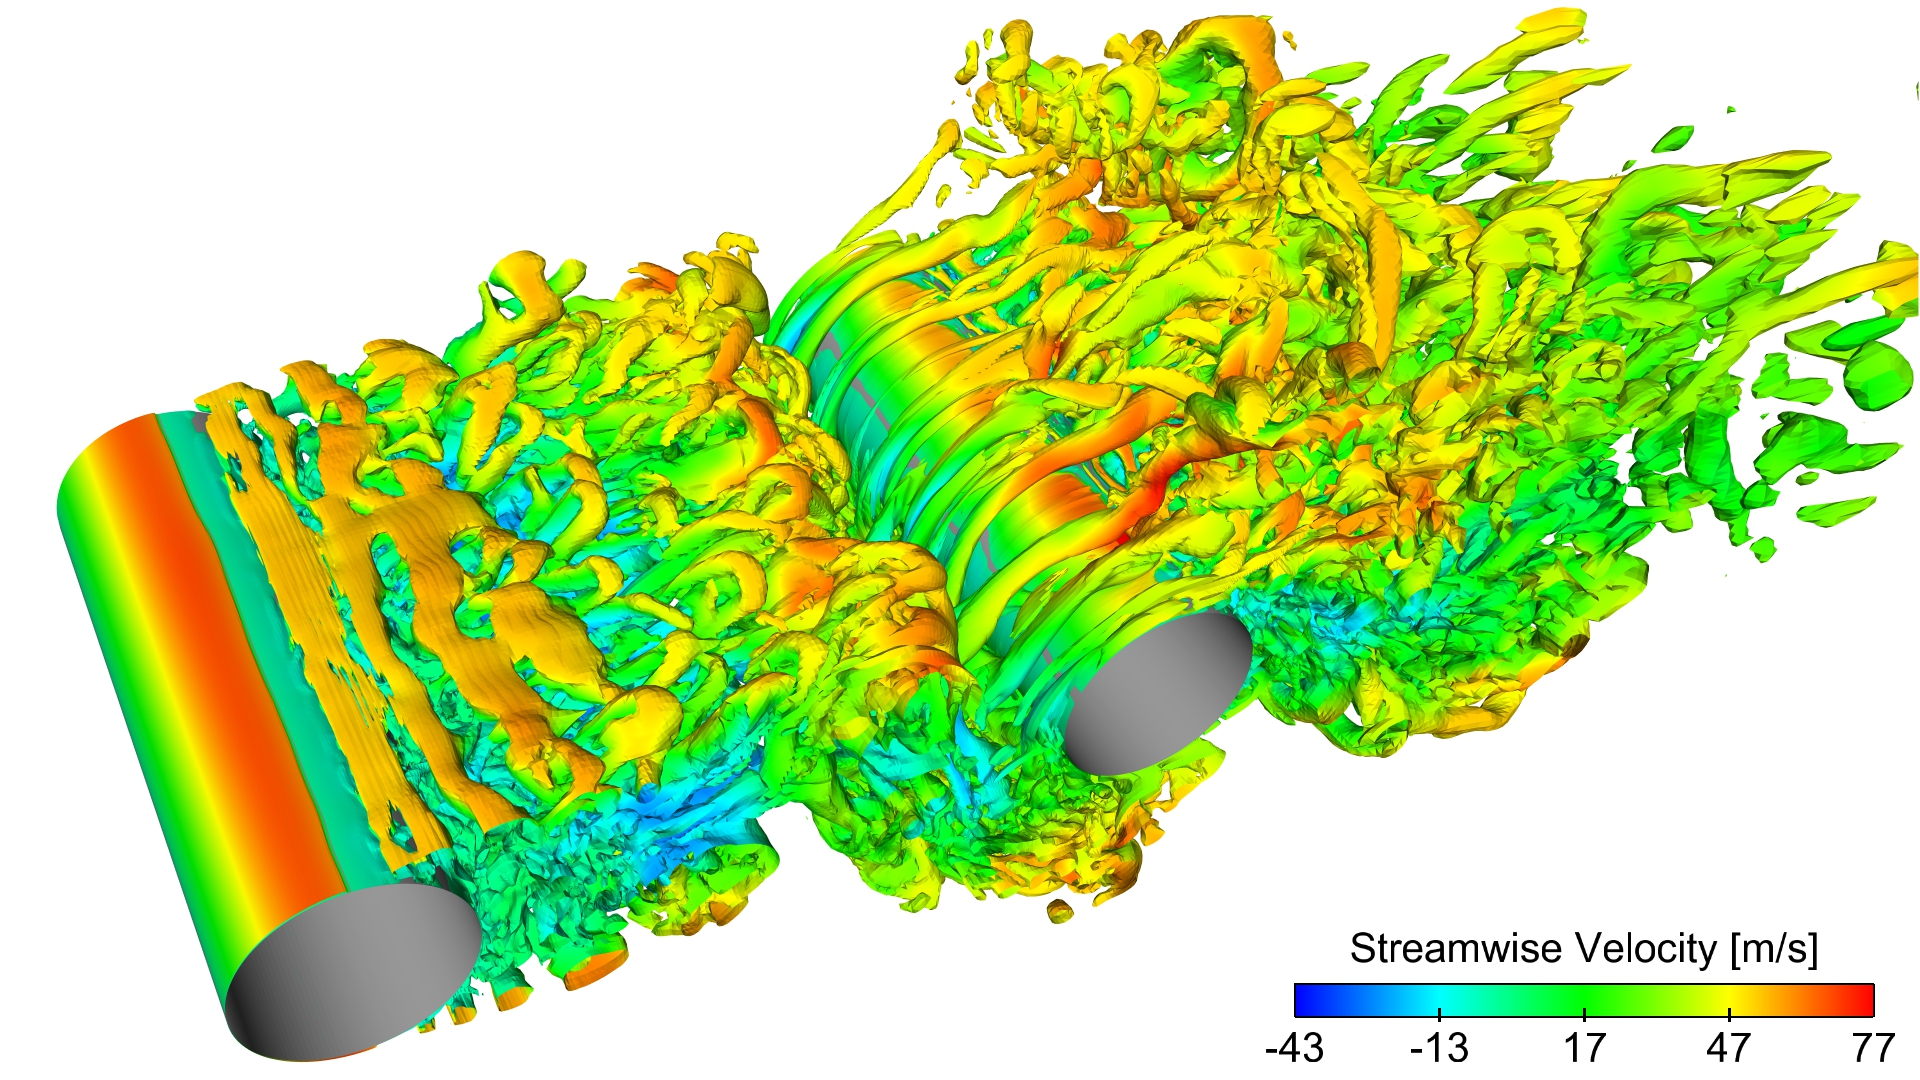
\includegraphics[width=0.45\textwidth]{ITC_Q_Criteria}
  \caption{Q判据等值面图}
  \label{fig:ITC_Q_Criteria}
\end{figure}
\end{verbatim}
\begin{figure}[!htbp]
  \centering
  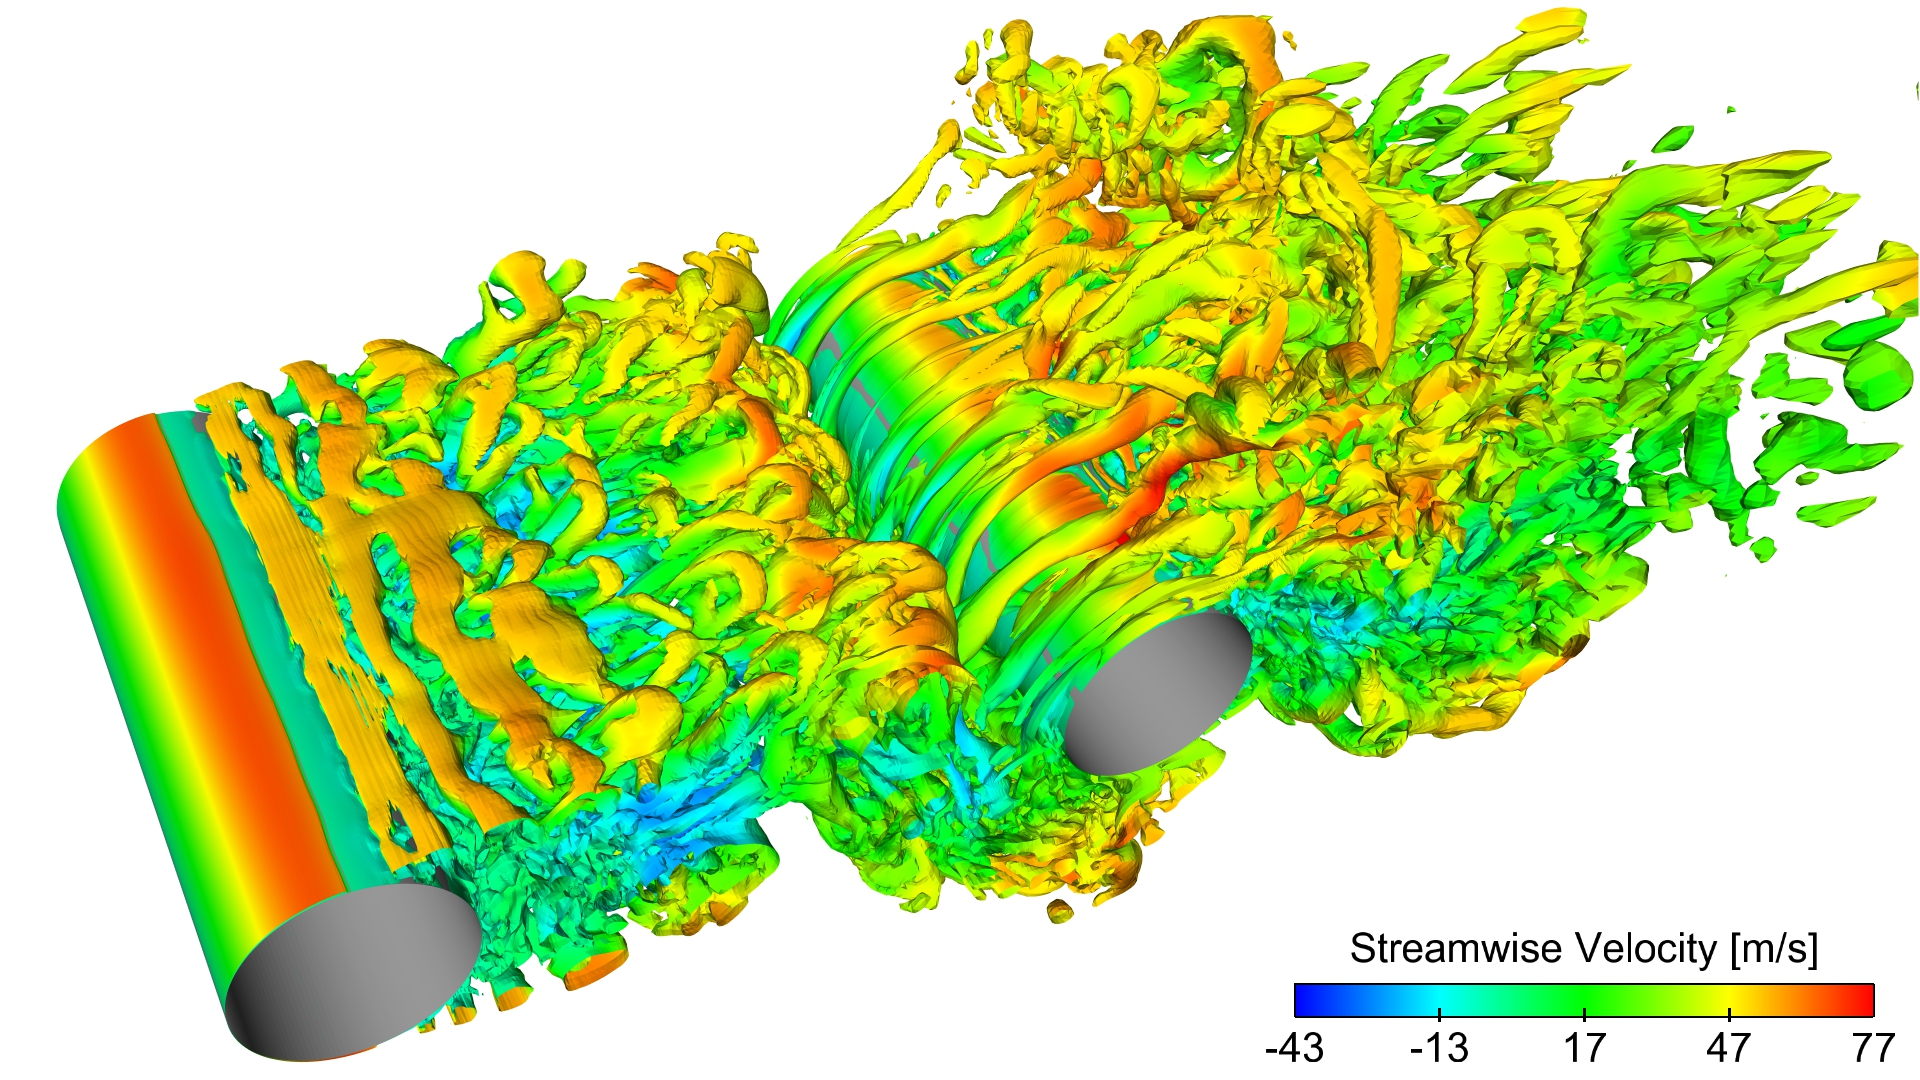
\includegraphics[width=0.45\textwidth]{ITC_Q_Criteria}
  \caption{Q判据等值面图}
  \label{fig:ITC_Q_Criteria}
\end{figure}

如果插图的空白区域过大,希望减少插入图片后的留白,以图片Y为例(图\ref{fig:Y}),可以使用如下代码模板:
\begin{verbatim}
\begin{figure}[!htbp]
  \centering
  %trim option's parameter order: left bottom right top
  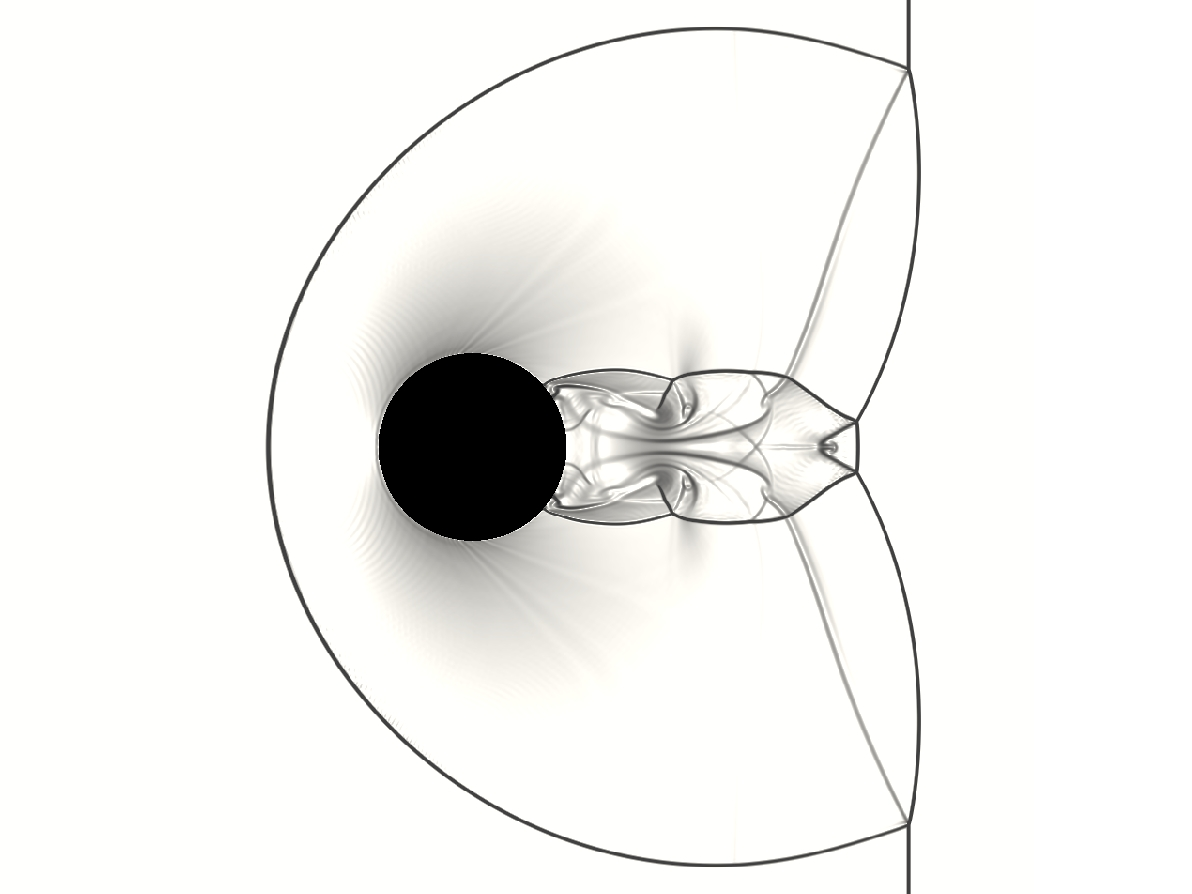
\includegraphics[trim = 30mm 0mm 30mm 0mm, clip, width=0.45\textwidth]{Y}
  \caption{Shock diffraction}
  \label{fig:Y}
\end{figure}
\end{verbatim}
\begin{figure}[!htbp]
  \centering
  %trim option's parameter order: left bottom right top
  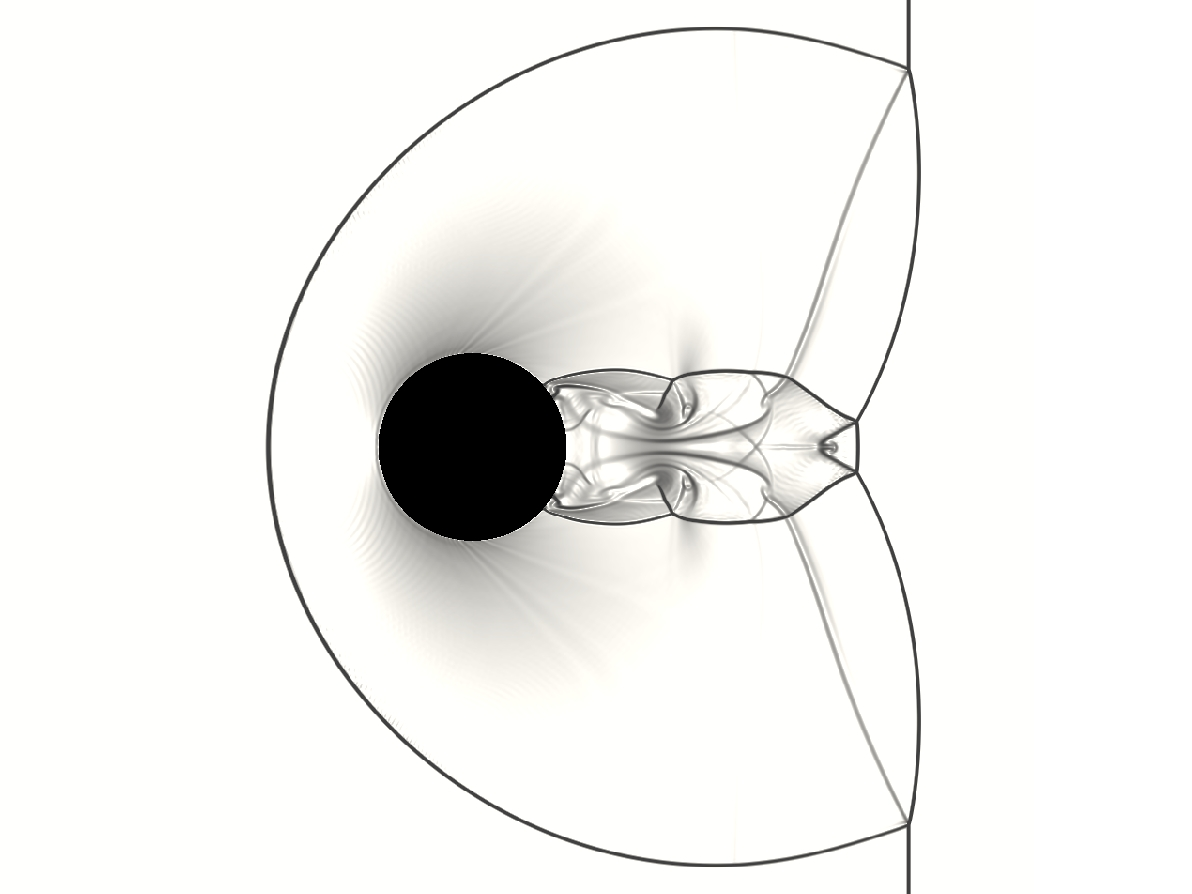
\includegraphics[trim = 30mm 0mm 30mm 0mm, clip, width=0.45\textwidth]{Y}
  \caption{Shock diffraction.}
  \label{fig:Y}
\end{figure}

多图的插入如图\ref{fig:HC_OASPL},其代码如下。
\begin{verbatim}
\begin{figure}[!htbp]
  \centering
  \begin{subfigure}[b]{0.45\textwidth}
    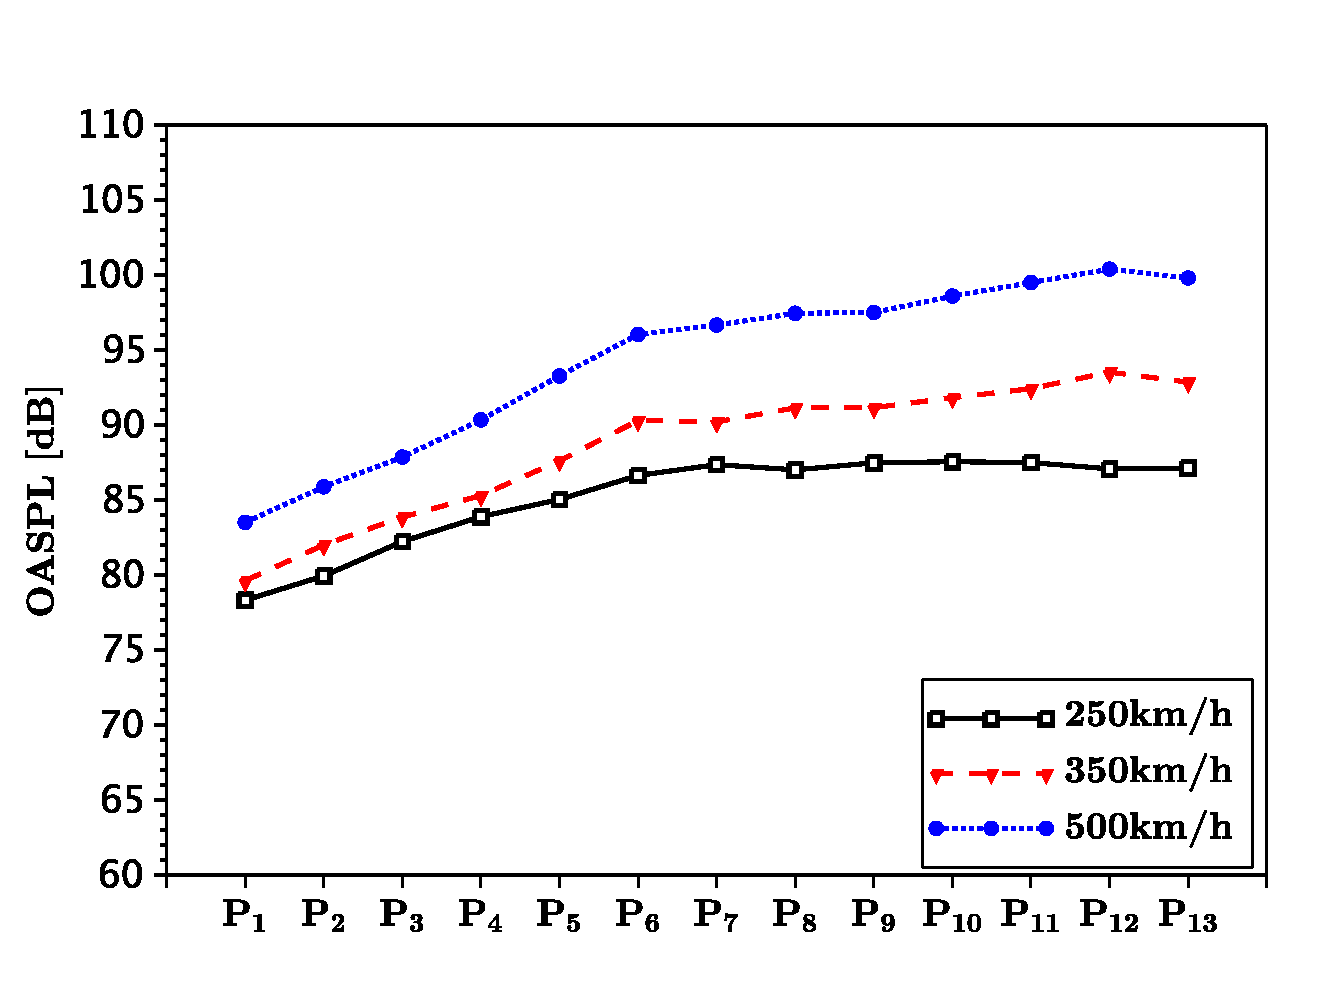
\includegraphics[width=\textwidth]{HC_OASPL_A}
    \caption{}
    \label{fig:HC_OASPL_A}
  \end{subfigure}%
  ~%add desired spacing
  \begin{subfigure}[b]{0.45\textwidth}
    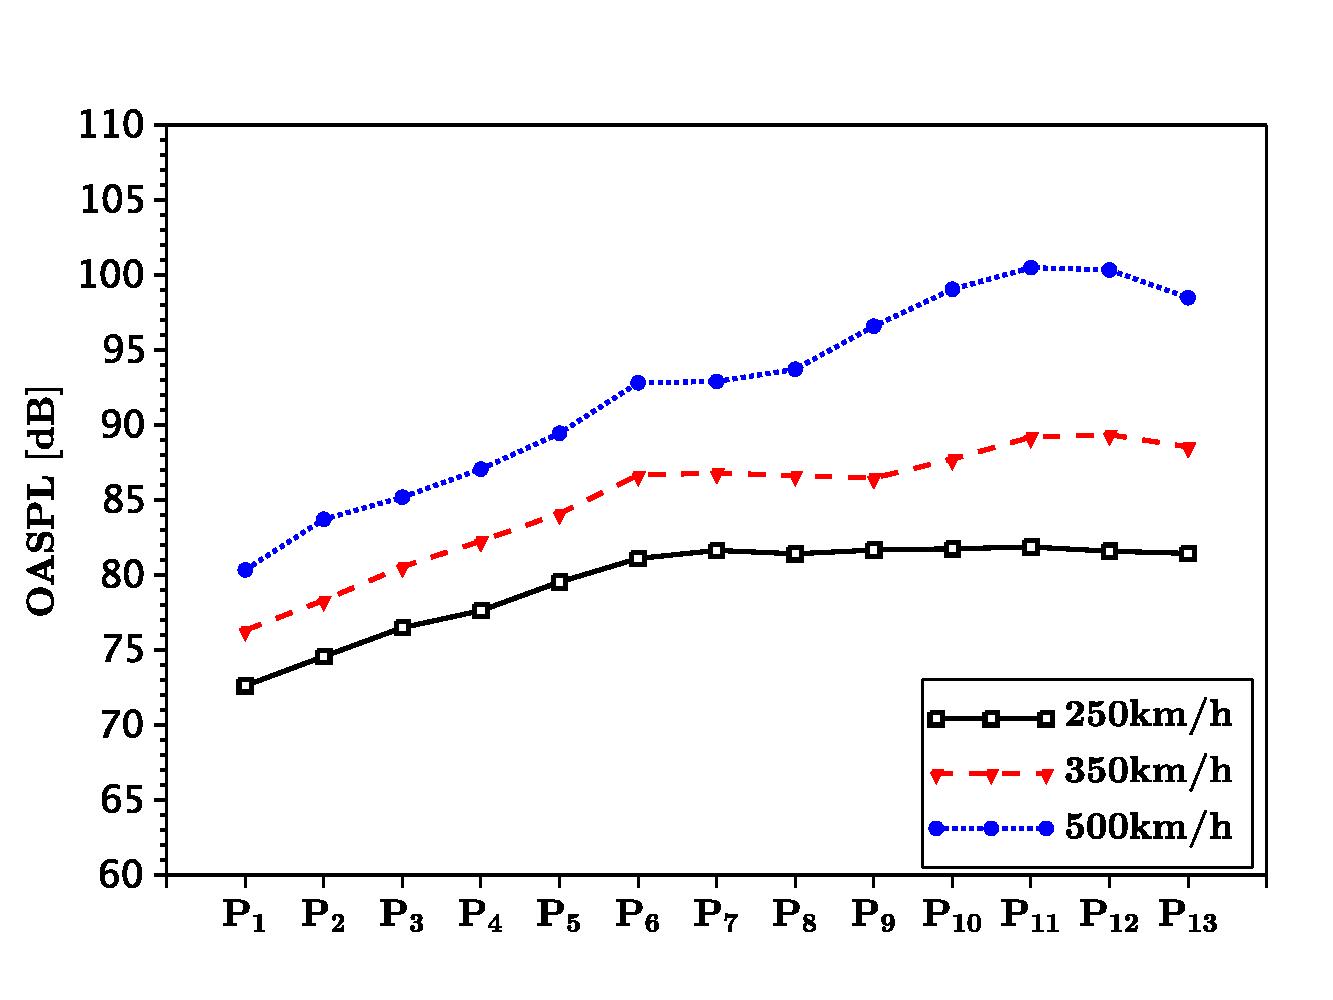
\includegraphics[width=\textwidth]{HC_OASPL_B}
    \caption{}
    \label{fig:HC_OASPL_B}
  \end{subfigure}
  \begin{subfigure}[b]{0.45\textwidth}
    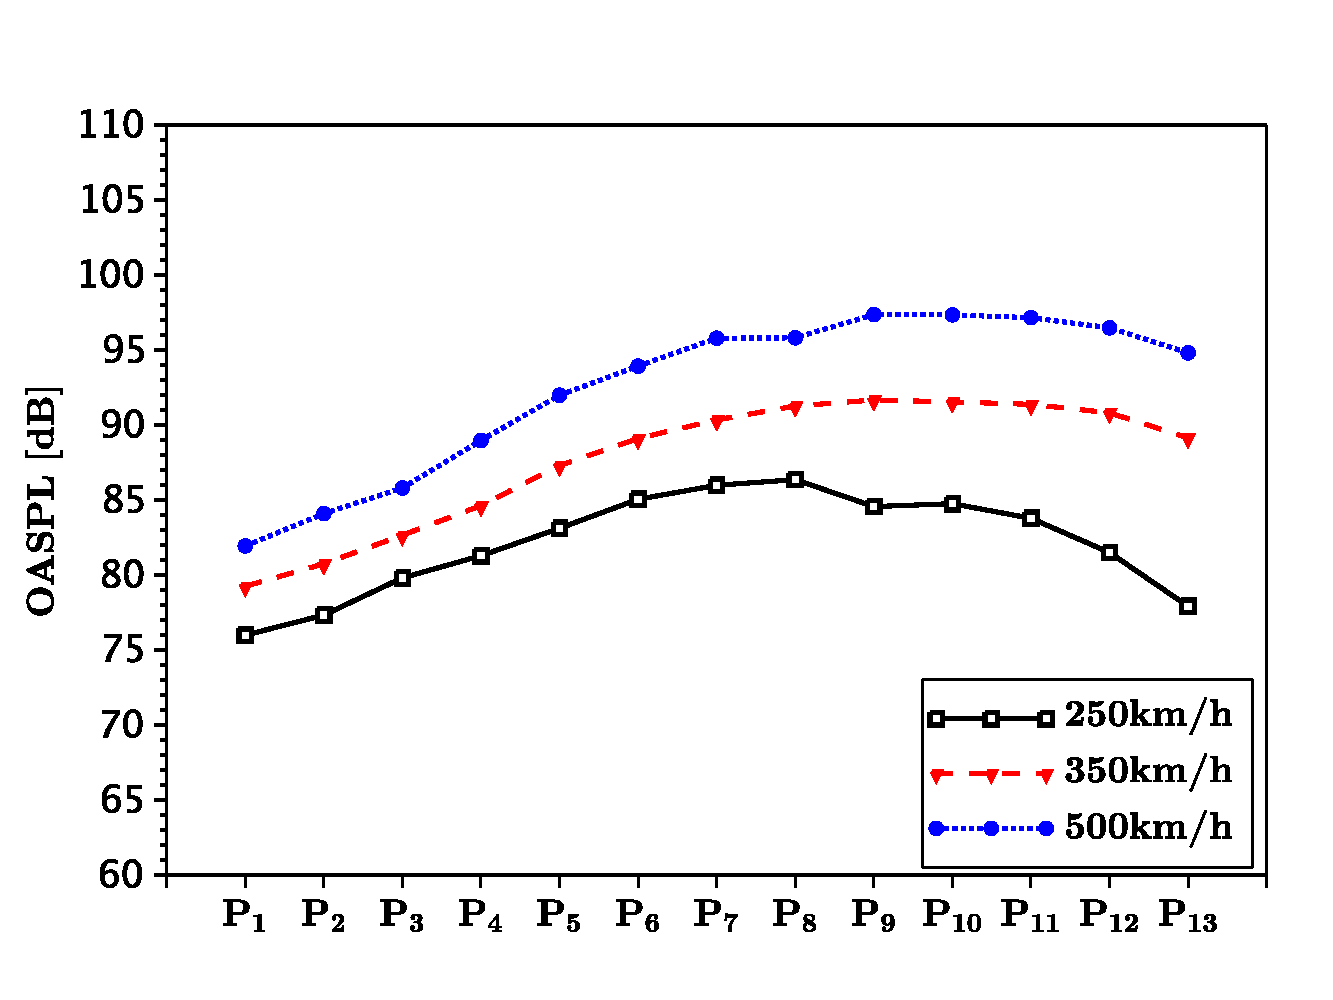
\includegraphics[width=\textwidth]{HC_OASPL_C}
    \caption{}
    \label{fig:HC_OASPL_C}
  \end{subfigure}%
  ~%add desired spacing
  \begin{subfigure}[b]{0.45\textwidth}
    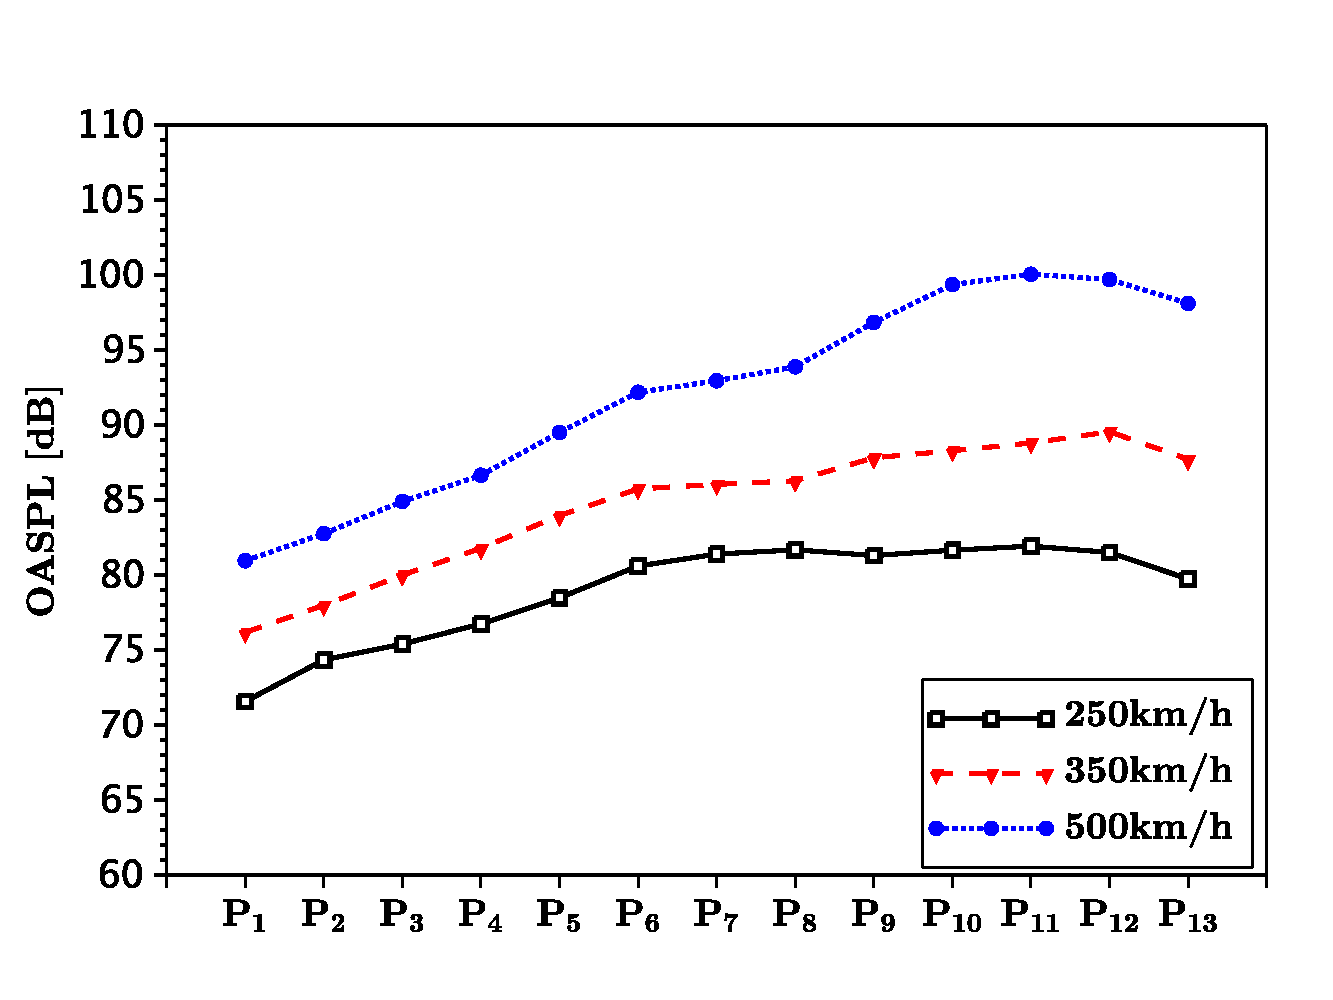
\includegraphics[width=\textwidth]{HC_OASPL_D}
    \caption{}
    \label{fig:HC_OASPL_D}
  \end{subfigure}
  \caption{总声压级。(a)$A$,(b)$B$,(c)$C$,(d)$D$}
  \label{fig:HC_OASPL}
\end{figure}
\end{verbatim}
\begin{figure}[!htbp]
  \centering
  \begin{subfigure}[b]{0.45\textwidth}
    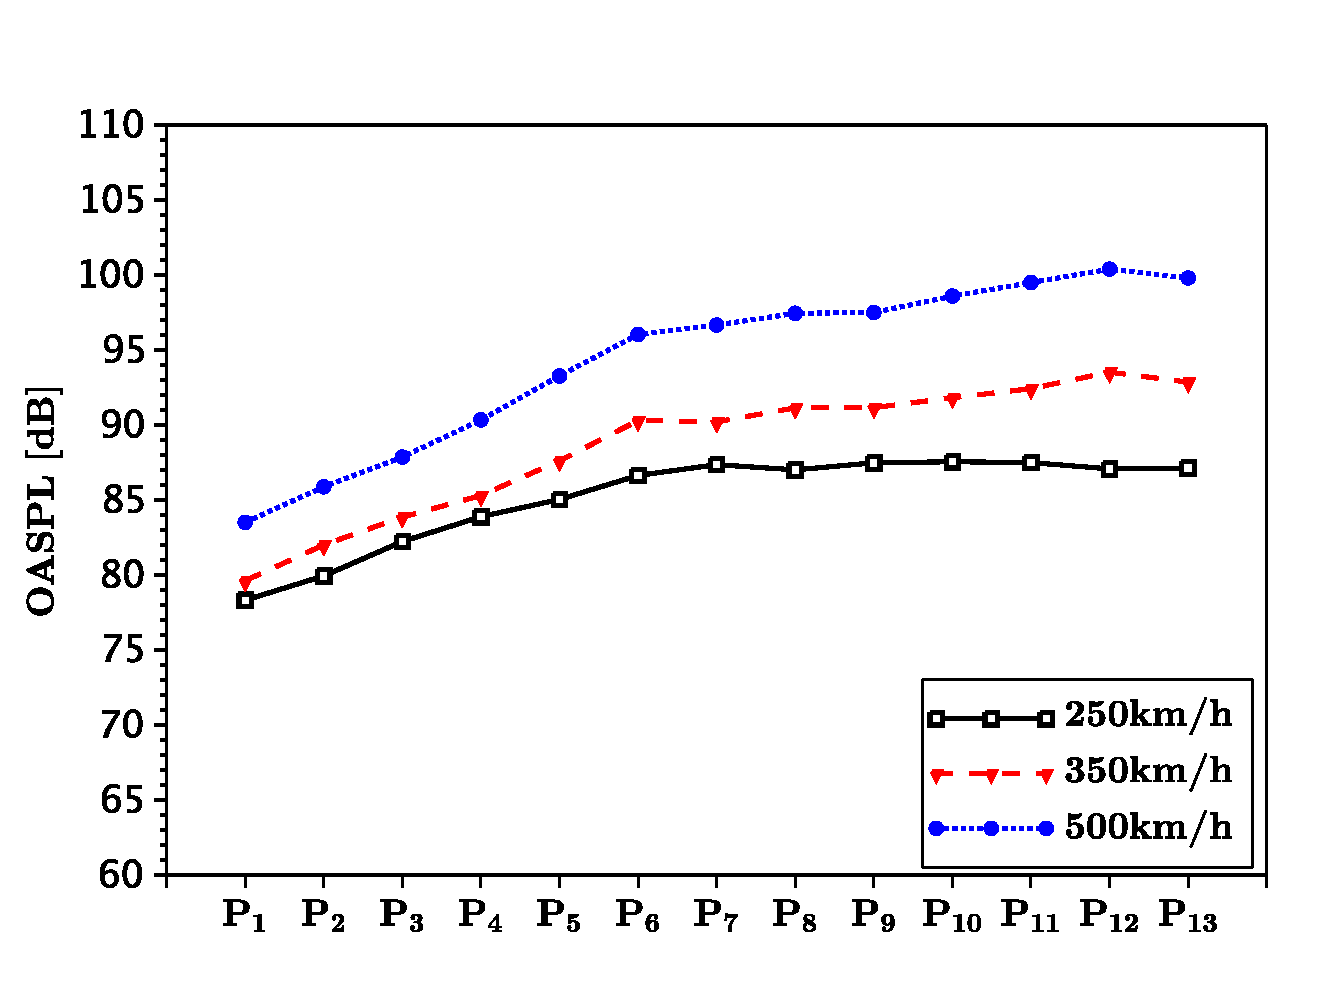
\includegraphics[width=\textwidth]{HC_OASPL_A}
    \caption{}
    \label{fig:HC_OASPL_A}
  \end{subfigure}%
  ~%add desired spacing
  \begin{subfigure}[b]{0.45\textwidth}
    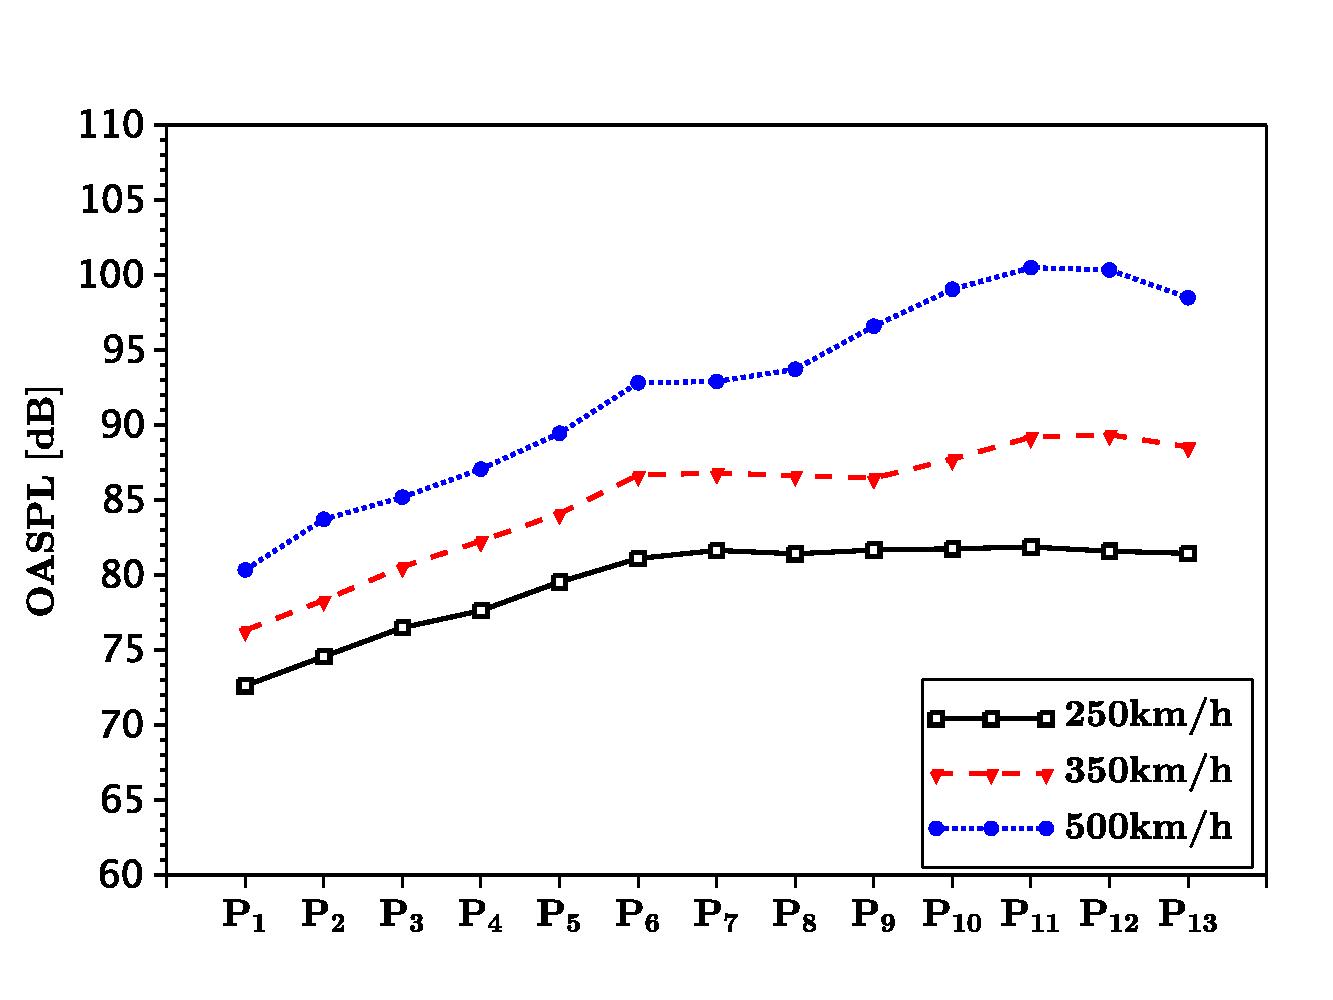
\includegraphics[width=\textwidth]{HC_OASPL_B}
    \caption{}
    \label{fig:HC_OASPL_B}
  \end{subfigure}
  \begin{subfigure}[b]{0.45\textwidth}
    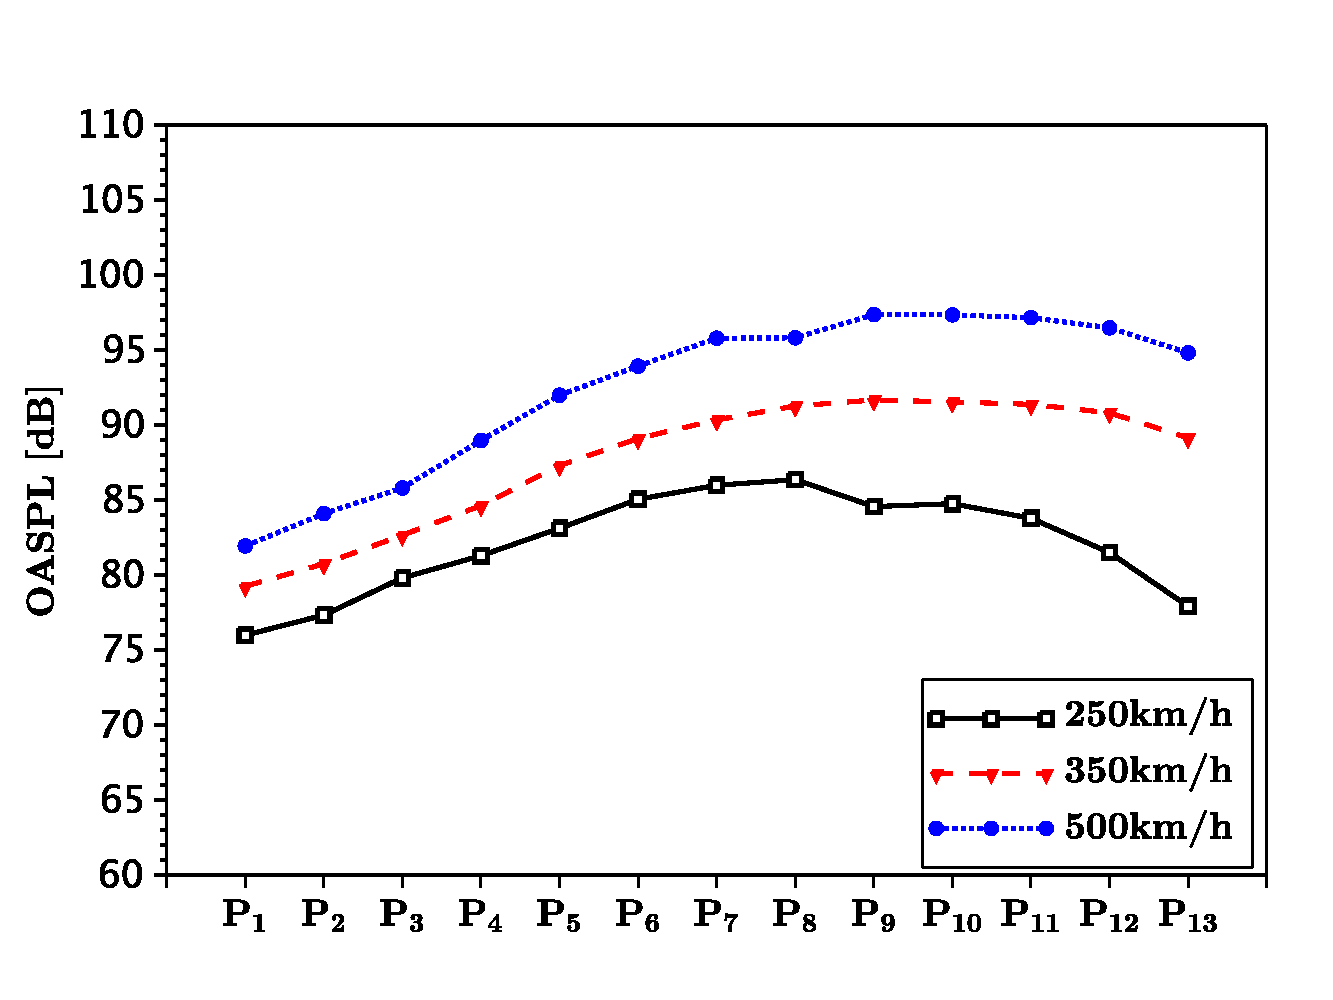
\includegraphics[width=\textwidth]{HC_OASPL_C}
    \caption{}
    \label{fig:HC_OASPL_C}
  \end{subfigure}%
  ~%add desired spacing
  \begin{subfigure}[b]{0.45\textwidth}
    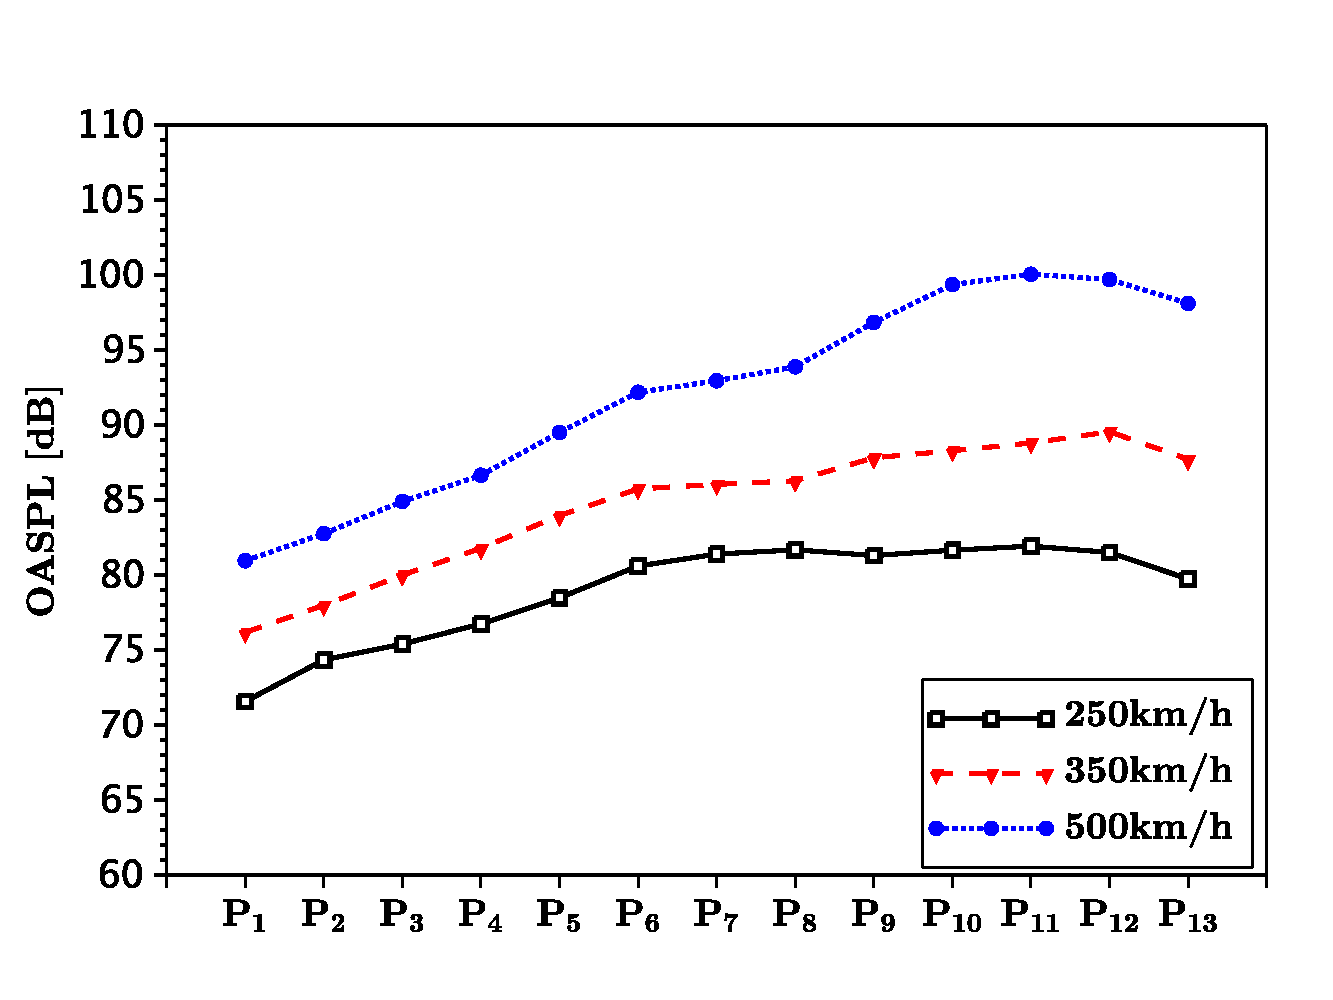
\includegraphics[width=\textwidth]{HC_OASPL_D}
    \caption{}
    \label{fig:HC_OASPL_D}
  \end{subfigure}
  \caption{总声压级。(a)$A$,(b)$B$,(c)$C$,(d)$D$}
  \label{fig:HC_OASPL}
\end{figure}

撰写论文中,插图和制表常用到的命令,已在\textbf{Useful Commands.txt}这个文本中给出了参考代码,大家只需copy使用即可。

\subsection{参考文献引用}

参考文献引用过程以实例进行介绍,假设需要引用名为Document Preparation System的文献,步骤如下:

1)使用google scholar搜索Document Preparation System,在目标条目下点击Cite,展开后选择Import into BibTeX打开此文章的BibTeX索引信息,将它们copy添加到ref.bib文件中(此文件位于Biblio文件夹下)。

2)你会发现索引信息中第一行为 \verb|@article{lamport1986document,|。其中 \verb|lamport1986document| 即为此文献的label (\textbf{中文文献也必须使用英文label},一般遵照:姓氏拼音+年份+标题第一字拼音的格式),想要在论文中索引此文献,有两种索引模式:

textual:\verb|\citet{lamport1986document}|。正如此处所示 \citet{lamport1986document}; 

parenthetical:\verb|\citep{lamport1986document}|。正如此处所示 \citep{lamport1986document}。

\textbf{多文献索引用英文逗号隔开}:

\verb|\citep{lamport1986document,chen2005zhulu}|。正如此处所示 \citep{lamport1986document,chen2005zhulu}

如此,即完成了文献的索引,请查看下本文档的参考文献一章,看看是不是就是这么简单呢?是的,就是这么简单!

不同文献样式和引用样式可在Thesis.tex中对commons.sty设置实现,如:

\verb+\usepackage[numbered]{commons}+ $\%$ default citation style. textual: Jones [1]; parenthetical: [1]

\verb+\usepackage[authoryear]{commons}+ $\%$ author year citation style. textual: Jones (1995); parenthetical: (Jones, 1995)

\verb+\usepackage[alpha]{commons}+ $\%$ alpha citation style. textual: not available; parenthetical: [Jon95]

若需将所有的上标改为嵌入式标注,则可在commons.sty 174行附近使用

\verb|\RequirePackage[square,comma,numbers,sort&compress]{natbib}|

的设置替换

\verb|\RequirePackage[square,comma,super,sort&compress]{natbib}|

如只希望在某些特定情形将上标改为嵌入式标注,则可使用

textural:\verb|\citepns{lamport1986document,chen2005zhulu}|。正如此处所示\citepns{lamport1986document,chen2005zhulu}

parenthetical:\verb|\citetns{lamport1986document,chen2005zhulu}|。正如此处所示\citetns{lamport1986document,chen2005zhulu}

参考文献索引更为详细的信息,请见Wikibook\citep{wikibook2014latex}。

\section{常见使用问题}

\begin{enumerate}
  \item 模板文档的编码为UTF-8编码。所有文件都必须采用UTF-8编码,否则编译后生成的文档将出现乱码文本。若出现文本编辑器无法打开文档或打开文档乱码的问题,请检查您使用的编辑器对UTF-8编码的支持,如果使用WinEdt作为文本编辑器,应在其

  options --》 Preferences --》 wrapping

  选项卡下将两种 Wrapping Modes 中的内容:

  TeX;HTML;ANSI;ASCII|DTX...

  修改为:

  TeX;\textbf{UTF-8|ACP;}HTML;ANSI;ASCII|DTX...

  同时,取消

  options --》 Preferences --》 Unicode

  中的Enable ANSI Format...选项。
  \item 推荐选择xelatex编译引擎编译。Compile.bat的默认设定为xelatex编译引擎。你也可以选择不使用此脚本编译,如直接使用 \TeX{}文本编辑器编译。注:\TeX{}文本编辑器编译的默认设定为pdflatex编译引擎,若选择xelatex编译引擎,请进入下拉菜单进行选择。为正确生成引用链接,编译步骤为: xelatex + bibtex + xelatex + xelatex。
  \item Texmaker使用简介
      \begin{enumerate}
          \item 使用 Texmaker 打开文档 Thesis.tex。
          \item 菜单 Options -> Define Current Document As 'Master Document'
          \item 菜单 User -> User Commands -> Edit User Commands -> Input Menu Item as 'Auto Build' -> Click 'wizard' -> add: xelatex + bibtex + xelatex + xelatex + pdf viewer -> Click 'OK'
          \item 使用 Auto Build 编译带有未生成引用链接的源文件,可以仅使用 xelatex 编译带有已经正确生成引用链接的源文件。
          \item 编译完成,View PDF,在pdf中'ctrl+click'可链接到相对应的源文件。
      \end{enumerate}
  \item 若编译过程中出现无法找到某些package的错误,如无法找到xcolor.sty,mathtools.sty,ctexbook.sty,newtext.sty等,\TeX{}编译程序一般可以自动下载和安装相应的文件,否则,请进入\LaTeX{}软件的Package Manager (Admin)确认启用Repository--Synchronize状态。下次编译过程中\TeX{}编译程序一般将自动下载安装\LaTeX{}宏包库。
  \item 模版在设计之初就尽可能地考虑了适应性。致谢,简历及攻读学位期间发表的学术论文与科研成果等几乎所有条目都是通过最为通用的
       
       \verb+\chapter{item name}+  and \verb+\section*{item name}+

       来显式实现的 (请仔细观察下Frontpage.tex, Prematter.tex, Backmatter.tex),从而你可以随意添加,放置,和修改他们,如同一般章节。对于图表目录名称则可在ucasthesis.cfg中进行修改。
   \item 设置正文行距: 在 custom.sty 99行附近, 修改

       \verb|\linespread{1.3}|

       设置参考文献行距: 在 custom.sty 103行附近, 修改/注掉

       \verb|\setlength{\bibsep}{0.0pt plus 0.3ex}|

       将subsection显示到目录当中: 在 custom.sty 107行附近, 将1改为2就可以了

       \verb|\setcounter{tocdepth}{1}% the depth for the Table of Contents.|

       如果需设置图2.3为图2-3,可将如下命令添加custom.sty中:

       \begin{verbatim}
\renewcommand{\theequation}{\arabic{chapter}-\arabic{equation}}
\renewcommand{\thefigure}{\arabic{chapter}-\arabic{figure}}
\renewcommand{\thetable}{\arabic{chapter}-\arabic{table}}
      \end{verbatim}
  \item 字体控制。如果对字体控制有较高需求,请选择xelatex编译引擎,并在commons.sty中设置需要的字体,如启用Times New Roman 作为英文字体,在commons.sty的105行附近设置:

      \verb+\setmainfont{Times New Roman}+
  \item 在某些情况下拷贝pdf文档内容到word时存在乱码。
      解决方式是选择安装adobe相应的字体库,请在公共网站(如百度云盘:\url{http://pan.baidu.com/share/home?uk=3188136325&view=share#category/type=0})搜索并下载如下四种中文字体文件:
      \begin{enumerate}
          \item AdobeFangsongStd-Regular.otf (adobe 仿宋)
          \item AdobeHeitiStd-Regular.otf(adobe 黑体)
          \item AdobeKaitiStd-Regular.otf(adobe 楷体)
          \item AdobeSongStd-Light.otf(adobe 宋体)
      \end{enumerate}
      下载字体文件后,双击安装相应字体。
      
      在Thesis.tex中设置启用adobe的字体:

      \verb+\documentclass[doublesided,fontset=adobe]{Style/ucasthesis}%+

      如果\LaTeX{}软件版本比较老旧,如Linux用户,ctex宏包没有更新,设置启用adobe的字体则为:

      \verb+\documentclass[doublesided,adobefonts]{Style/ucasthesis}%+
     
     最后选择xelatex编译引擎编译。

     因为模版的设定考虑兼顾不同操作系统(Windows, Linux, Mac OS)并兼顾pdflatex和xelatex,为了模版的健壮性,上述方案并未作为原始设定。
 \item 页眉页脚的设定在commons.sty的底部。始于323行附近的frontmatterstyle,mainmatterstyle,和backmatterstyle分别用于定义前言,主要内容,和附录的页眉页脚样式。一般默认情况下每一章的第一页不应显示页眉页脚,若想修改此行为,请将377-379行附近的plain样式定义注空即可。即修改为

\begin{verbatim}
\fancypagestyle{plain}{%
    %\fancyhf{}% clear fields
    %\renewcommand{\headrulewidth}{0pt}% header rule
    %\renewcommand{\footrulewidth}{0pt}% footer rule
}
\end{verbatim}
     
     关于页眉页脚各个命令的作用和意义请参见fancyhdr的用户文档 \url{https://www.ctan.org/pkg/fancyhdr?lang=en}。如果需要在页眉页脚中添加章节字样,请使用
      \begin{enumerate}
          \item \verb+\CTEXthechapter+  显示: 第X章
          \item \verb+\CTEXthesection+  显示: 第X节
      \end{enumerate}
      参见ctex宏包用户文档 \url{http://ctan.mirror.rafal.ca/language/chinese/ctex/ctex.pdf}
  \item 一般规范下,每一章应开始于奇数页。从而若前一章结束于奇数页,则一空白页将被插入以保证上述规则。如果想修改规则以取消空白页,有如下三种方案:
\begin{itemize}
    \item 在thesis.tex的documentclass中使用singlesided替代doublesided选项。这一命令使文档不区分奇偶页,因此章可以开始于任意页。此方案将移除所有的空白页,包括封面处的。同时,页面页脚的设定不再区分奇偶页。
    \item 可以在ucasthesis.cls文件中106行附近,将cleardoublepage命令的定义修改为:

      \verb|\def\cleardoublepage{\clearpage}|

      这一命令使产生空白页的机制失效。这一方案将移除所有的空白页,包括封面处的。但与方案一不同的是,页面页脚的设定可以区分奇偶页。
  \item 在thesis.tex的documentclass中添加openany选项(openany与doublesided和printcopy都可搭配)。这一命令使章可以开始于任意页。同时,将custom.sty中86行和thesis.tex中88行附近的cleardoublepage改为clearpage。此方案将移除所有的用于调整章的起始位置的空白页,而不包括封面处的。同时,页面页脚的设定可以区分奇偶页。
\end{itemize}
      无论哪种方案都需要注意对页眉页脚的影响并做出合适的调整。个人的推荐是采用默认设置,尽量避免将精力花在这些无关紧要的细节上。\LaTeX{}的特点是标准化,而其导致的问题则是任何脱离标准的修改都将花费相当的精力。对于电子档的论文,在thesis.tex的documentclass中,若不想使用doublesided,则可使用singlesided来减少空白页。而对于打印版,启用printcopy选项以替换doublesided/singlesided选项,这样可使奇偶页的排版在打印装订后更美观。
  \item 若pdflatex编译出现pdfTeX error (font expansion): auto expansion is only possible with scalable fonts。是因为MikTex安装后字体配置异常,请进入软件的package manager更新你的\LaTeX{}宏包库,并请进入
      
      \verb+C:\Program Files\MiKTeX 2.9\miktex\bin\x64+

       找到并运行updmap.exe。
    \item 部分同学留意到一个所谓的新的模板要求,那个模板是一位学生发布的,而其英文封面的设定不满足中国科学院大学学位论文封面设定。因中国科学院大学学位论文撰写规定只是限定了封面格式但是没有要求具体的内容格式,部分所因为图方便省事就直接将其作为了模板发布到了所内。但是,迄今为止学校官网上的撰写规定和模板(\url{http://onestop.ucas.edu.cn/home/info/abc167cb-4589-4e05-b014-052fa9291d0c/1})未做出任何修改,亦未发表任何官方声明表示模板需要修改。所以,当前模板将不会在官方版发布之前做出调整。
\end{enumerate}

\nocite{*}% show all the bibliography entries

\part{增强学习}
\chapter{增强学习简介} \label{chap:introduction}


这部分是对Masashi Sugiyama的《Statistical Reinforcement Learning: Modern Machine Learning Approaches》的笔记。


增强学习试图解决未知环境下的决策问题。增强学习可以概括为:两个要素( \textbf{环境}, \textbf{玩家}),三种信号( \textbf{状态}, \textbf{行动}, \textbf{反馈})。在一个未知的环境下,玩家基于\textbf{策略}选择行动,之后,环境更新状态,并给予玩家反馈。基于环境和玩家的互动,在没有任何指令的情况下,玩家也可以完成指定任务。通常情况下,我们通过马尔可夫决策过程来建模增强学习任务。在任一离散时间$t$,玩家观察到环境状态信号$s_t \in S$,给出其行动信号$a_t \in A$,相应的,环境更新状态信号$s_{t+1} \in S$,给出即时反馈信号$r$.
$$r_t = r(s_t,a_t,s_{t+1})$$
状态信号属于状态空间,行动信号属于行动空间。$r(s_t,a_t,s_{t+1})$ 是即时反馈方程。

环境的初始状态$s_1$符合概率分布。如果状态空间是离散的,则初始概率分布可以通过概率质量函数计算$P(s)$
$$0 \leq P(s) \leq 1 \quad  \forall s \in S $$
$$\sum_{s \in S } P(s) = 1$$
如果状态空间是连续的,则初始概率分布可以通过概率密度函数计算
$$ p(s) \geq 0 \quad  \forall s \in S $$
$$\int_{s \in S} p(s) ds = 1 $$
事实上,概率质量函数可以通过概率密度函数计算(基于Dirac Delta Function),因此,之后我们只关注连续的状态空间。
$$p(s) = \sum_{s^\prime \in S} \delta(s^\prime - s)P(s^\prime)$$
环境的动态变化可以用条件概率密度表达成状态的转化概率分布(transition probability distribution)
$$p(s^\prime|s,a) \geq 0 \quad  \forall s,s^\prime \in S \quad  \forall a \in A $$
$$\int_{s^\prime \in S} p(s^\prime|s,a) ds^\prime = 1  \quad  \forall s \in S \quad  \forall a \in A $$
玩家通过\textbf{策略}$\pi$来决定行动。当采取确定策略行动时,我们可以把策略看成状态的函数。
$$\pi(s) \in A \quad  \forall s \in S $$
行动空间可以是离散的也可以是连续的。
当处理比较复杂的增强学习问题时,随机策略是更好的选择。此时,在某一状态下,玩家的行动选择存在概率分布。随机策略可以表达成行动和状态的条件概率。
$$\pi(a|s) \geq 0 \quad  \forall s \in S \quad  \forall a \in A $$
$$\int_{a \in A} \pi(a|s) da  = 1  \quad  \forall s \in S $$
随机策略可以帮助玩家更好的探索环境的所有状态。玩家和环境的一系列互动([状态,行动])被称为\textbf{经历}。

互动的次数可以是有限的,也可以是无限的。在此,我们只关注有限互动的增强学习任务。一次经历$h$可以被表达成
$$ h = [s_1,a_1,\dots,s_T,a_T,s_{T+1} $$

一次经历的\textbf{回报}$R$是衰减累计反馈。
$$R(h) = \sum_{t=1}^T\gamma^{t-1}r(s_t,a_t,s_{t+1})$$
$\gamma$ 是衰减因子。

增强学习的目的是发展出最佳策略$\pi_*$



\section{系统要求}

\texttt{ucasthesis}宏包可以在目前大多数的\TeX{}编译系统中使用,例如C\TeX{}、MiK\TeX{}、\TeX{}Live。推荐的\TeX{}编译系统 + 文本编辑器为
\begin{itemize}
    \item Linux: \TeX{}Live + vim or Texmaker
    \item MacOS: \TeX{}Live or Mac\TeX{} + Macvim or Texmaker
    \item Windows: \TeX{}Live or Mik\TeX{}  + Texmaker
\end{itemize}
\TeX{}编译系统 (如MiK\TeX{}、\TeX{}Live) 用于提供编译环境,文本编辑器 (如Texmaker、vim) 用于编辑\TeX{}源文件。

\section{问题反馈}

\begin{center}
莫晃锐 (mohuangrui) \quad mohuangrui@gmail.com

模版下载地址: \url{https://github.com/mohuangrui/ucasthesis}
\end{center}

欢迎大家反馈模板不足之处,一起不断改进模板。希望大家向同事积极推广\LaTeX{},一起更高效地做科研。

%%% ++++++++++++++++++++++++++++++++++++++++++++++++++++++++++++++++++++++++++++++++++
%
%%%%% --------------------------------------------------------------------------------
%%
%%%%******************************** Appendix ****************************************
%%
%% Some subordinate chapters.
\cleardoublepage
\appendix%

\chapter{中国科学院大学学位论文撰写要求}
学位论文是研究生科研工作成果的集中体现,是评判学位申请者学术水平、授予其学位的主要依据,是科研领域重要的文献资料。根据《科学技术报告、学位论文和学术论文的编写格式》(GB/T 7713-1987)、《学位论文编写规则》(GB/T 7713.1-2006)和《文后参考文献著录规则》(GB7714—87)等国家有关标准,结合中国科学院大学(以下简称“国科大”)的实际情况,特制订本规定。

\section{学位论文的一般要求}

学位论文必须是一篇(或由一组论文组成的一篇)系统的、完整的学术论文。学位论文应是学位申请者本人在导师的指导下独立完成的研究成果,除论文中已经注明引用的内容外,不得抄袭和剽窃他人成果。对学位论文研究做出重要贡献的个人和集体,均应在文中以明确方式标明。学位论文的学术观点必须明确,且立论正确,推理严谨,数据可靠,层次分明,文字正确、语言通畅,表述清晰,图、表、公式、单位等符合规范要求。

\section{学位论文的水平要求}

硕士学位论文要选择在基础学科或应用学科中有价值的课题,对所研究的课题有新的见解,并能表明作者在本门学科上掌握了坚实的基础理论和系统的专门知识,具有从事科学研究工作或独立担负专门技术工作的能力。

博士学位论文要选择在国际上属于学科前沿的课题或对国家经济建设和社会发展有重要意义的课题,要突出论文在科学和专门技术上的创新性和先进性,并能表明作者在本门学科领域掌握了坚实宽广的基础理论和系统深入的专门知识,具有独立从事科学研究工作的能力。

\section{撰写学位论文的语言及文字}

除外国来华留学生及外语专业研究生外,研究生学位论文一般应采用国家正式公布实施的简化汉字撰写;应采用国家法定的计量单位。学位论文中采用的术语、符号、代号在全文中必须统一,并符合规范化的要求。

外国来华留学生可用中文或英文撰写学位论文,但须采用中文封面,且应有详细的中文摘要。外语专业的学位论文等应用所学专业相应的语言撰写,摘要应使用中文和所学专业相应的语言对照撰写。

为了便于国际合作与交流,学位论文亦可有英文或其它文字的副本。

\section{学位论文的主要组成部分}

学位论文一般由以下几个部分组成:中文封面、英文封面、致谢、中文摘要、英文摘要(Abstract)、目录、正文、参考文献、附录、作者简历及攻读学位期间发表的学术论文与研究成果。

\begin{enumerate}
  \item 学位论文题目应当简明扼要地概括和反映出论文的核心内容,一般不宜超过25个汉字(符),英文题目一般不应超过150个字母,必要时可加副标题。

  \item 论文摘要包括中文摘要和英文摘要(Abstract)两部分。论文摘要应概括地反映出本论文的主要内容,主要说明本论文的研究目的、内容、方法、成果和结论。要突出本论文的创造性成果或新见解,不宜使用公式、图表,不标注引用文献。英文摘要(Abstract)应与中文摘要内容相对应。摘要最后另起一行,注明本文的关键词(3-5个),关键词是为了文献标引工作从论文中选取出来,用以表示全文主题内容信息的单词或术语。

  \item 正文是学位论文的主体,包括引言(或绪论)、论文主体及结论等部分。
    \begin{itemize}
      \item 引言(或绪论)应包括选题的背景和意义,国内外相关研究成果述评,本论文所要解决的问题、所运用的主要理论和方法、基本思路和论文结构等。引言应独立成章,用足够的文字叙述,不与摘要雷同。

      \item 论文主体由于涉及不同的学科,在选题、研究方法、结果表达方式等有很大的差异,不作统一的规定。但必须严格遵循本学科国际通行的学术规范,言之成理,论据可靠,实事求是,合乎逻辑,层次分明,简练可读。

      \item 结论是对整个论文主要成果的总结,应明确、精炼、完整、准确。结论应明确指出本研究的创新点,对论文的学术价值和应用价值等加以预测和评价,说明研究中尚难解决的问题,并提出今后进一步在本研究方向进行研究工作的设想或建议。应严格区分本人研究成果与他人科研成果的界限。
    \end{itemize}

  \item 参考文献应本着严谨求实的科学态度,凡学位论文中有引用或参考、借用他人成果之处,均应按不同学科论文的引用规范,列于文末(通篇正文之后)。需正确区分直接引用和转引并明确加以标注。

  \item 学位论文印刷及装订要求:学位论文用A4标准纸打印、印刷或复印,按顺序装订成册。自中文摘要起双面印刷,之前部分单面印刷。论文必须用线装或热胶装订,不使用钉子装订。学位论文封面采用国科大统一规定的学位论文封面格式,封面用纸一般为150克(需保证论文封面印刷质量,字迹清晰、不脱落),博士学位论文封面颜色为红色,硕士学位论文封面颜色为蓝色。

  \item 学位论文的提交、保存与使用:学位申请者需按规定向国科大提交学位论文的印刷本和电子版,印刷本和电子版在内容与形式上应完全一致;国科大有权保存学位论文的印刷本和电子版,并提供目录检索与阅览服务,可以采用影印、缩印、数字化或其它复制手段保存学位论文;研究所、国科大有义务保护论文作者的知识产权。涉密学位论文在解密后,须按此规定执行。

  \item 本规定自印发之日起施行【2013年04月07日】,解释权属于校学位评定委员会,由国科大学位办公室负责解释。原《中国科学院研究生院研究生学位论文撰写规定》(院发学位字〔2012〕31号)同时废止。
\end{enumerate}
%
%%%%% --------------------------------------------------------------------------------
%%
%%%%******************************* Backmatter ***************************************
%%
%% Matters of Bibliography, Glossary, Index.
\backmatter
%%
%%% >>> Bibliography
%%
\intotoc{\bibname}% add a corresponding item to the contents table and bookmark
\bibliography{Biblio/ref}%
%%
%%% >>> Other contents
%%
%%
%%% >>> Resume and Published papers
%%
\chapter{作者简历及攻读学位期间发表的学术论文与科研成果}

\section*{CASthesis~作者基本情况}

吴凌云,男,福建省屏南县人,1975 年出生,中国科学院数学与系统科学研究院博士研究生。

\section*{联系方式}

通讯地址:北京市~2734 信箱,中科院数学与系统科学研究院应用数学所

邮编:100080

E-mail: aloft@ctex.org

\section*{ucasthesis~作者基本情况}

莫晃锐,男,湖南省湘潭县人,1989 年出生,中国科学院力学研究所硕士研究生。

\section*{联系方式}

通讯地址:北京市北四环西路15号中国科学院力学研究所

邮编:100190

E-mail: mohuangrui@gmail.com

\section*{攻读学位期间发表的学术论文及科研成果}

[1] Thesis Template of the University of Chinese Academy of Sciences, 2014.

\section*{项目资助情况}

可以随意添加新的条目或是结构

%%
%%% >>> Acknowledgements
%%
\chapter{致\quad 谢}

值此论文完成之际,谨在此向多年来给予我关心和帮助的老师、学长、同学、
朋友和家人表示衷心的感谢!

没有~ctex package~的众多前辈的辛勤付出和~CASthesis package~作者吴凌云学长的贡献,
~\LaTeX{}~菜鸟的我是无法完成此学位论文模板的。在~\LaTeX{}~中的一点一滴的成长源于
开源社区的众多资料和教程,在此对所有前辈们的付出表示感谢!

......

谨把本文献给我最敬爱的父亲!

%%
\end{document}
%%%%% --------------------------------------------------------------------------------
